\chapter{Background}
\label{bckgrnd}

This chapter presents some general information on stereo vision that be useful for understanding the decision that were made in developing this stereo vision system.

\section{Computer Stereo Vision}

Computer vision is concerned with using computers to understand and use information that is within visual images~\cite{computerVision}. There are many different types of computer vision, which range from using one image to multiple images to obtain information. One image is not enough to determine the three dimensional properties of the objects within the image.

Stereo vision uses multiple images of the same scene in order to construct a three dimensional representation of the objects in the images~\cite{stereoVision}. Comparing multiple images together for their similarities and differences allows for the depth to be obtained.

Binocular stereo~\cite{binocularStereo} involves comparing a pair of images. These images are normally acquired simultaneously from a scene. By searching for corresponding pairs of pixels between the two images, depth information can be determined~\cite{binocularStereo}. Pixel based comparisons can require substantial amount of computational power and time. Certain assumptions are made because of the computational resources required. Camera calibration and epipolar lines [cite 14-14 and define better] are common assumptions. For example, two images of the same scene are 640 x 480 pixels in size. Each image therefore contains 307,200 pixels, which is over 600,000 pixels between the two images for one frame. For a real-time application, say 30 frames per second for example, that becomes over 18 million pixels between the two images that would need to be processed every second.

Computational requirements for real-time applications can be reduced in several ways. First, by lowering the number of pixels in the images reduces the number of pixel comparison per second. Images at a size of 320 x 240 pixels would require a quarter of the number of computations at the cost of losing some amount of detail in the images. Also, reducing the number of frames per second will decrease the amount of computing needed. Going much below 30 frames per second is noticeable to a person and can be annoying to observe a slow frame rate. A robot on the other hand, depending on its task and how fast its moving, might only need a few frames per second in order to function within a desired range. So image resolution could be more important than frames per second for a robot if details are more important than speed.

Figure~\ref{fig:sv_diagram} below represents a simplified illustration of binocular stereo vision. The two cameras are held at a known fixed distance from each other and are used to triangulate different the distance of objects in the images they create. The points U\textsubscript{L} and U\textsubscript{R} in the left and right images, respectively, are 2D represents the point P that is in 3D space. By comparing the offset of between U\textsubscript{L} and U\textsubscript{R} in the two images, it is possible to obtain the distance of point P away from the cameras~\cite{stereoVisionDiagram}.

\begin{figure}
	\begin{center}
		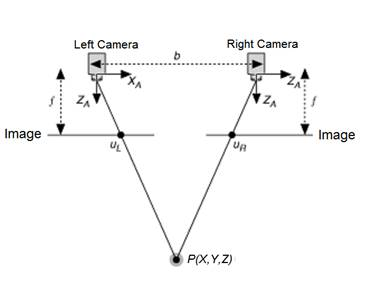
\includegraphics{figures/stereoVisionDiagram.jpg}
		\captionfonts
		\caption{Simplified binocular stereo vision system~\cite{stereoVisionDiagram}.}
		\label{fig:sv_diagram}
	\end{center}
\end{figure}

The closer an object is to the stereo vision system, the greater the offset of corresponding pixels will be. If an object is too close to the system, it is possible for one camera to see part of an object that the other camera cannot. The farther an object is away from the stereo vision system, the smaller the offset of corresponding pixels will be. If an object is far enough away, it is possible for an object to be in almost the exact same location in both images. You can show this to yourself by holding a finger up close to your face, close one eye, and then alternate between which eye is open and which eye is closed. Your finger should appear to move a noticeable amount. Next, hold your finger as far away from you as you can and again alternate between which eye is open and which is closed. You should notice that your finger appears to move significantly less than it did when your finger was close to your face. That is how stereo vision works. The distance of an object is inversely proportional to the amount of offset between the two images.

\subsection{Parallelism in Stereo Vision}

Processing images for stereo vision allows for a high degree of parallelism. Locating the corresponding position of a pair of pixels is independent of finding another corresponding pair of pixels. This independent nature allows for the ability to process different parts of the same images at the same time, if there is hardware to support it.

Field Programmable Gate Arrays (FPGAs) allow for parallel processing to be implemented of the images. In Section~\ref{sec:impl} the amount of parallel processing used for the modular stereo vision system presented in this paper is discussed. 

\section{Stereo Vision Algorithms}

Stereo vision algorithms can be placed into one of three different categories: pixel-based methods, area-based methods, and feature-based methods~\cite{similarAlgorithms}. Pixel-based methods utilize pixel by pixel comparisons. They can produce dense disparity \textbf{(define!)} maps, but at the cost of higher computation complexity and higher noise sensitivity~\cite{similarAlgorithms}. Area-based methods utilize block by block comparisons. They can also produce dense disparity maps and are less sensitive to noise, however, accuracy tends to be low in areas that are not smooth~\cite{similarAlgorithms}. Feature-based methods utilize features, such as edges and lines for comparisons. They cannot produce dense disparity maps, but have a lower computational complexity and are insensitive to noise~\cite{similarAlgorithms}. 

There are a lot of stereo vision algorithms out there~\cite{taxonomy}. In the taxonomy of~\cite{taxonomy}, 20 different stereo vision algorithms were compared against each other using various reference images. Many algorithms are based on either the sum of absolute differences (SAD) or correlation algorithms~\cite{alteraStratixIVPaper}.

An algorithm that is similar to SAD is Sum of the Square Differences (SSD). Both of these algorithms produce similar results and contain around the same amount of error~\cite{similarAlgorithms}. SAD was chosen over the other algorithms to implement because it is simpler to implement in hardware. SSD requires squaring the difference between corresponding pixels and summing it up. Since squaring a number is the number multiplied by itself, the number will be added to itself that many times to produce the squared value. This is a lot more over head, and more hardware, than just taking the absolute difference of the difference of each corresponding pair.

\subsection{Sum of the Absolute Differences Algorithm}

SAD is a pixel-based matching method~\cite{alteraStratixIVPaper}. Stereo vision uses this algorithm to compare a group of pixels called a window from one picture with a window in another picture. The SAD algorithm, shown in Equation~\ref{eq:sadAlg1}~\cite{alteraStratixIVPaper}, takes the absolute difference between each pair of corresponding pixels and sums all of those values together to create a SAD value. One SAD value by itself does not give any useful information about those two corresponding windows. Several SAD values will be calculated from different candidate windows for each reference window. Out of the all the SAD values calculated for the reference window, the SAD value with the smallest value (all of them are positive because of the absolute part in the equation) is determined to contain the matching pixel. Figure~\ref{fig:sad_corr} shows for one reference window, there are several candidate windows used. The line that the candidate windows move across are called epipolar lines. 

\begin{equation}
	\sum\limits_{(i,j)\in W}\left| I_{1}(i,j)-I_{2}(x+i,y+j) \right|
	\label{eq:sadAlg1}
\end{equation}

\begin{figure}
\begin{center}
	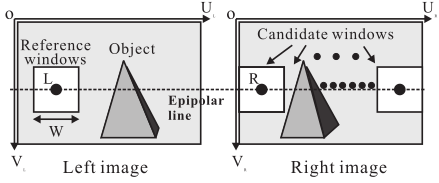
\includegraphics{figures/sadCorrespondingWindows.png}
	\captionfonts
	\caption{Searching for corresponding points between the two images~\cite{sadParallel}.}
	\label{fig:sad_corr}
\end{center}
\end{figure}

In stereo vision, epipolar lines are created from the two cameras capturing images from the same scene. Figure~\ref{fig:epipolar} show the epipolar line that point X must be on in the corresponding images. This is useful because if the epipolar lines are known for both images, then it is possible to know the line that two corresponding points are on. It reduces the problem of finding the the same two points from a 2D area to a 1D line. Now, if the epipolar lines in both images are horizontal as they are in Fig.~\ref{fig:sad_corr} as opposed to them being at a diagonal as they are in Fig.~\ref{fig:epipolar} then Eq.~\ref{eq:sadAlg1} reduces to Equation~\ref{eq:sadAlg2}. For cameras that are not perfectly aligned, rectification is often used in order to align epipolar lines between images~\cite{rectification}. However, many stereo vision algorithms will assume that the epipolar lines are rectified to simplify the overall processing required.

\begin{figure}
\begin{center}
	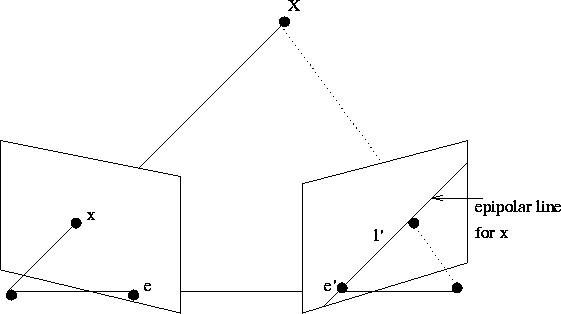
\includegraphics[height=50mm]{figures/epipolar.png}
	\captionfonts
	\caption{The epipolar line that point X is on for both images~\cite{epipolar}.}
	\label{fig:epipolar}
\end{center}
\end{figure}

\begin{equation}
	\sum\limits_{(i,j)\in W}\left| I_{1}(i,j)-I_{2}(x+i,j) \right|
	\label{eq:sadAlg2}
\end{equation}

The disparity is the amount of offset between two corresponding pixels. The disparity range is the range that the candidate window will move through the image and is represented by the value 'x' in Eq.~\ref{eq:sadAlg2}. It corresponds to the amount of SAD values that will be calculated. Figure~\ref{fig:sadGraphs} shows two types of SAD search methods. Fig.~\ref{fig:globalSAD} selects the overall SAD value with the lowest value to be the matching pixel. However, Fig.~\ref{fig:localSAD} limits the search region to a specific area. This helps to avoid issues of similar looking areas that are not near the reference window from being falsely identified as matching. The downside to this is that if an object gets too close, meaning it would have high disparity values, and if the search region is not large enough, then the objects distance will be miss classified. It is important to determine a window size and a search region that are not too small and are not too big.

\begin{figure}
\begin{center}
	\begin{subfigure}{0.4\textwidth}
		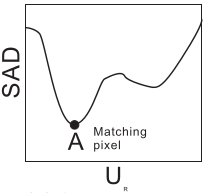
\includegraphics[width=\textwidth]{figures/sadGlobalGraph.png}
		\caption{Global SAD search}
		\label{fig:globalSAD}
	\end{subfigure}
	\begin{subfigure}{0.4\textwidth}
		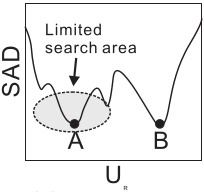
\includegraphics[width=\textwidth]{figures/sadLocalGraph.png}
		\caption{Local SAD search}
		\label{fig:localSAD}
	\end{subfigure}
	\captionfonts
	\caption{The SAD between a reference window and several candidate windows~\cite{sadParallel}.}
	\label{fig:sadGraphs}
\end{center}
\end{figure}

For example, Figure~\ref{fig:windows} shows a template window (Figure~\ref{fig:template}) from one image and the search area (Figure~\ref{fig:search}) in the other window. The disparity range is three, or zero to two. There are three 3x3 windows within the search region in Fig.~\ref{fig:search}. From left to right the three search windows have the center pixel as 4, 6, and 5, respectively. 

Comparing corresponding pixels in the template window with the first search window (let's call it S0) gives the absolute differences for all nine pixels going from left to right and top to bottom of 8, 1, 1, 2, 1, 0, 1, 2, and 2. So the SAD value for S0 of 18 is obtained by adding up all nine of those values. The SAD value for the second search window (S1) is 6 and the last search window (S2) is 13. The template window has the smallest difference between S1, which means that the center pixel in S1 is determined to be the corresponding pixel for the center pixel in the template window. 

The disparity value is 1 (how far the matching search window was shifted to the left). The disparity value is used to create a disparity map. Each disparity value in the disparity map is at the same relative location that the center pixel of its corresponding template window is located.

\begin{figure}
\begin{center}
	\begin{subfigure}{0.3\textwidth}
		\begin{center}				
			\begin{tabular}{|l|c|r|}
				\hline
				1 & 2 & 3 \\\hline
	  			4 & 5 & 6 \\\hline
		    	7 & 8 & 9 \\
		    	\hline
			\end{tabular}
		\end{center}
		\caption{Template Window}
		\label{fig:template}
	\end{subfigure}
	\begin{subfigure}{0.3\textwidth}
		\begin{center}		
			\begin{tabular}{|l|c|c|c|r|}
				\hline
				9 & 1 & 2 & 4 & 5 \\\hline
		  		2 & 4 & 6 & 5 & 3 \\\hline
		    	8 & 6 & 7 & 8 & 7 \\
		    	\hline
			\end{tabular}
		\end{center}
		\caption{Search Region}
		\label{fig:search}
	\end{subfigure}
	\captionfonts
	\caption{Template (reference) window and search (candidate) window.}
	\label{fig:windows}
\end{center}
\end{figure}
